The creation of the present temporal Knowledge Graph, which comprises a subset of the larger CoyPu KG, involves several steps to integrate the data into a structured and standardized framework. 

First, the source data is retrieved manually from the corresponding web services in a machine-readable format. Next, the data is converted into RDF format using an ontology schema that defines the relevant concepts, properties, and relationships. This enables the representation of the source data as a set of triples and allows for its integration with other RDF data sources. 
Both the ALCED and GTA datasets are mapped to RDF based on custom ontology declarations. These declarations contain the specific semantic specifications of transforming the source data into triples and form an extension of the central CoyPu COY ontology \cite{coy_2023}. 
We provide both the ontology OWL files, as well as the RML mapping rules used for the graph creation process in our repository for reproducibility.

\begin{description}
\item[Simplification] We aim to simplify the ACLED and GTA datasets to extract relevant information for our use case, while minimizing noise from irrelevant information. Thus, for GTA, we exclude triples that contain labels, intervention and state acts IDs, and event types, as these triples do not provide any additional information. For ACLED, we exclude triples with comments and labels, and only consider the country location of each event.

\item[Aggregation]
GTA uses the hierarchical industry classification schemes \textit{CPC 2.1} and \textit{HS 2012} to denote the affected sectors and products of an intervention. These schemes may include a very large number of categories, making the analysis more challenging. To address this issue, we use broader sector and product categories, based on higher-level groupings within the respective classification scheme. E.g., instead of considering each individual product category, we group products into broader categories based on their use or production process, such as "primary agricultural products". This is useful for modeling the impact of political violence or other events on trade flows, as it helps to identify the most affected sectors or products. 
As this data reduction is helpful in our use case but could be harmful in others, it is a configurable step during dataset generation.  
\item[Merging GTA and ACLED] The GTA and ACLED events can be linked via their annotated country information. In GTA, country data is available for the implementing and the affected jurisdiction of each intervention or state act. Meanwhile, in ACLED, country information is available from the locations of involved actors and of the ACLED events themselves. We illustrate such a connection in Figure~\ref{fig:link}, depicting two ACLED events and a GTA intervention in Ukraine and Russia in 2021. It is important to note that this link does not necessitate causality, but rather serves as a foundation for further analysis.

\begin{figure}
    \centering
    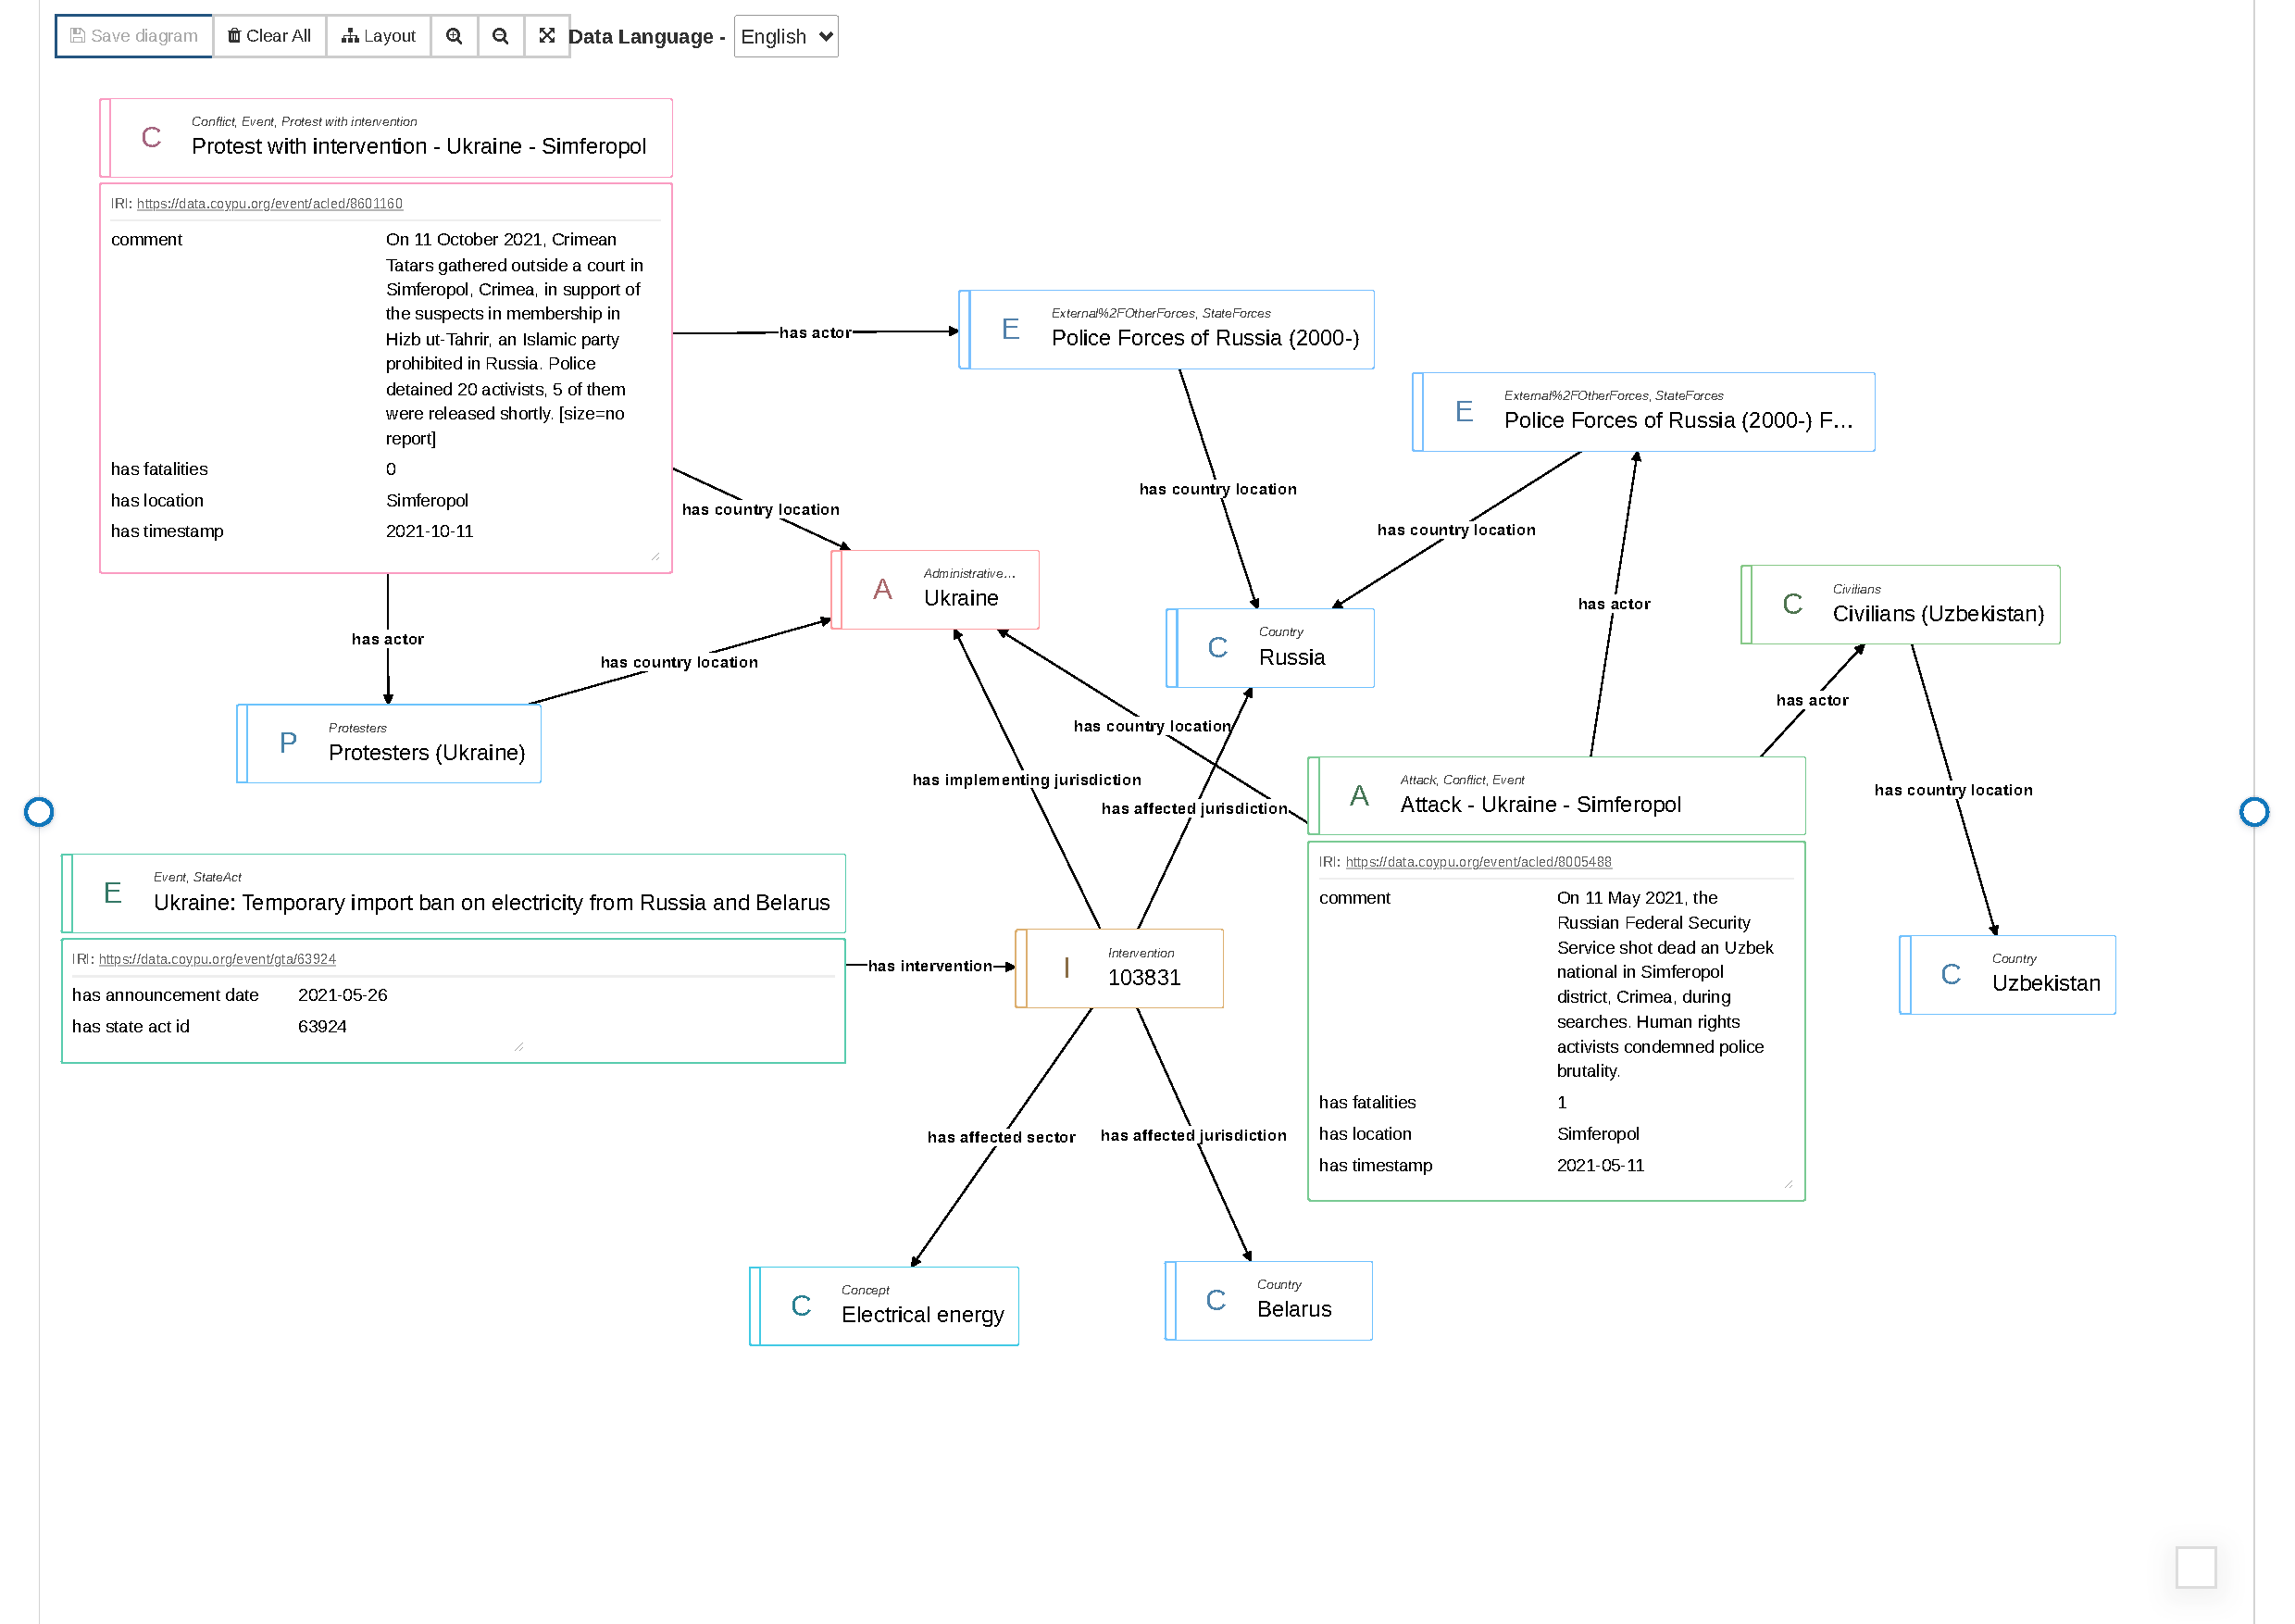
\includegraphics[clip, trim=1.1cm 5.0cm 1.2cm 1.8cm, width=0.7\textwidth]{figs/acled_gta.pdf}
    \caption{Link between two ACLED events and a GTA event via locations in 2021. The ACLED events (\textit{Attack - Ukraine - Simferopol}, green, and \textit{Protest with intervention - Ukraine - Simferopol}, pink) and the GTA intervention (\textit{intervention 103831}, yellow) link via Russia and Ukraine. }
    \label{fig:link}
\end{figure}

\item[Temporal Information] 
From the given graph in RDF format, we create a tKG with daily granularity, containing quadruples for each day in the year 2021. We have opted to utilize quadruples as our chosen representation, as they are widely employed in the field of tKG forecasting research, see e.g., \cite{Jin2019oldrenet}, \cite{Li2021regcn}, \cite{Han2021xerte}.
ACLED provides daily timestamps for each event. We create the quadruples by adding this timestamp data to all triples that are connected to this event. 
GTA provides an announcement date of each state act, as well as the implementation date, and - if existing - the removal date for each connected intervention. 
Since our use case (see Section~\ref{sec:UseCase}) aims to predict upcoming global trade events, we focus on the earliest available date for each GTA event, i.e. the announcement date. Therefore, we add the announcement date timestamp to all triples belonging to a state act or intervention. 
The output of this step is a tKG with quadruples in TXT format for further analysis. 
\end{description}
